\section*{RESULTS}\label{sec:results}

Data from two roll decay model tests conducted at zero speed were
available. These tests where analyzed by fitting a cubic model to the model test data. The two models were very similar in terms of roll damping and stiffness (see fig.\ref{fig:mdl}), suggesting
good repeatability in the model tests as well as in the parameter
identification technique (PIT) used. The individual damping from each oscillation obtained with the logarithmic decrement method are very scattered, but this does not seem to influence the two models for the 0 speed case, which are very similiar.


Data from one roll decay model tests conducted at a ship speed corresponding to 15.5 knots full scale ship speed was also available (see fig.\ref{fig:mdl}). This model tests was analyzed in the same way as the other tests. It was found that the damping was higher at speed. The ship got a small yaw rate at the end of test, giving a small steady roll angle due to the centrifugal force. Since this effect is not included in the mathematical
model used, the steady roll angle was instead removed by removing the linear trend in the roll angle signal.

    \begin{figure}[h]
        \begin{center}
        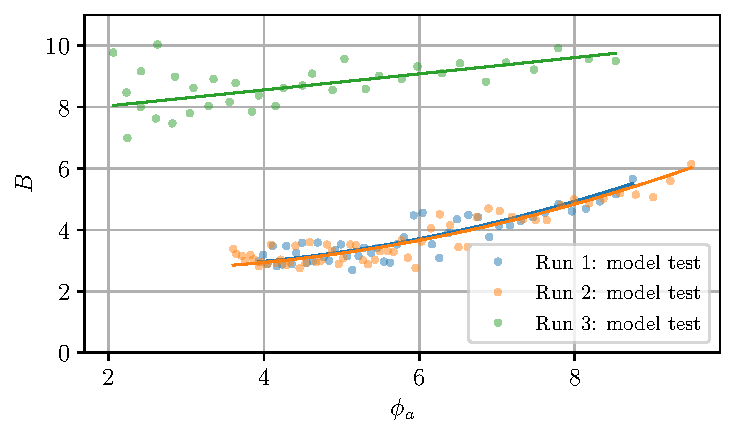
\includegraphics[width = 0.4\textwidth]{figures/mdl.pdf}
        \end{center}
        \vspace{-1cm}
        \caption{Model test results}
        \label{fig:mdl}
    \end{figure}
    
\subsection*{Results for 0 knot}\label{knots}

When looking at predictions for KVLCC2 at 0 speed made with regular Ikeda's method, it was found that the eddy damping $B_E$ was too high compared with the regular implementation, compared to the model test results. Even though the rest of the components would also be overpredicted, the $B_E$ would still be too large. The eddy damping calculated with $C_r$ predicted with the descision tree gave much better agreement.

    \begin{figure}[h]
        \begin{center}
        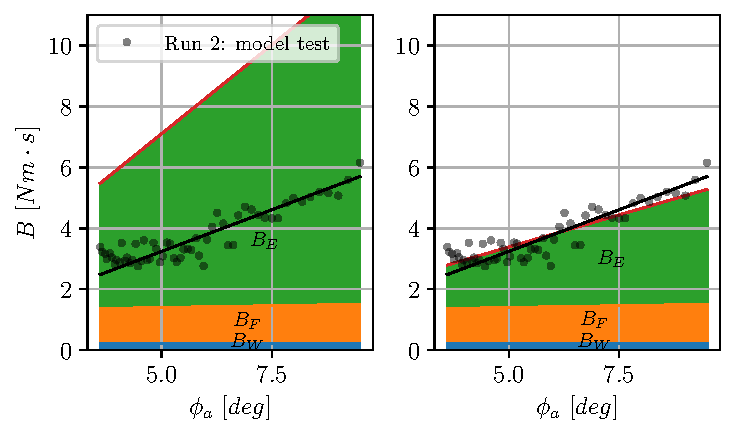
\includegraphics[width = 0.4\textwidth]{figures/ikeda.pdf}
        \end{center}
        \vspace{-1cm}
        \caption{Ikeda prediction}
        \label{fig:ikeda}
    \end{figure}
    
Replacing the wave damping $B_W$, for the zero speed case above, with values obtained with FNPF is shown below. The total damping from the hybrid method is similar to the model test results for the zero speed case. 

    \begin{figure}[H]
        \begin{center}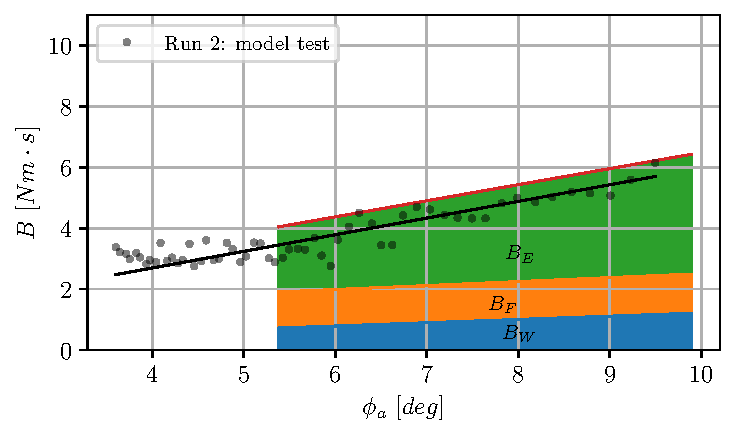
\includegraphics[width = 0.4\textwidth]{figures/hybrid_0.pdf}
        \end{center}
        \vspace{-1cm}
        \caption{Roll damping from Hybrid method (0 kn)}
        \label{fig:hybrid_0}
    \end{figure}   


\subsection*{Results for 15.5 knots}\label{knots}

Simulations of roll decay were conducted with FNPF for each model test case. The results from these simulations can be seen in the figure below.

    \begin{figure}[H]
        \begin{center}
        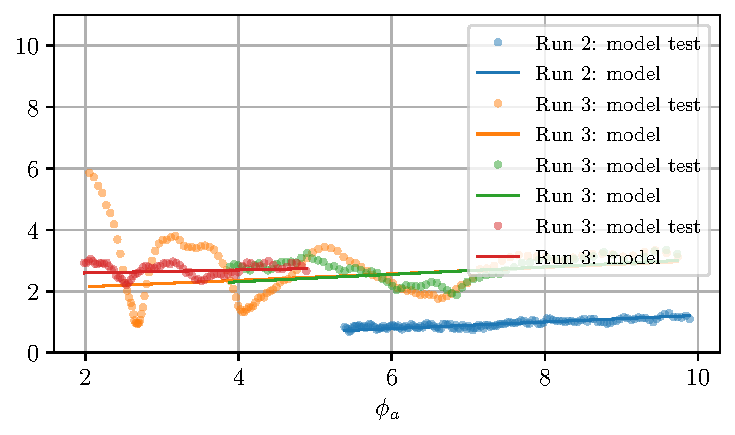
\includegraphics[width = 0.4\textwidth]{figures/fnpf.pdf}
        \end{center}
        \vspace{-1cm}
        \caption{Wave damping component from FNPF}
        \label{fig:fnpf}
    \end{figure}
    
The wave damping from FNFP seems to be reasonably linear at zero speed according the figure above, which is in line with Ikeda's assumption for the derivation of eddy damping \cite{7505983/4AFVVGNT}.

For the in speed case the agreement is however even better:

    \begin{figure}[H]
        \begin{center}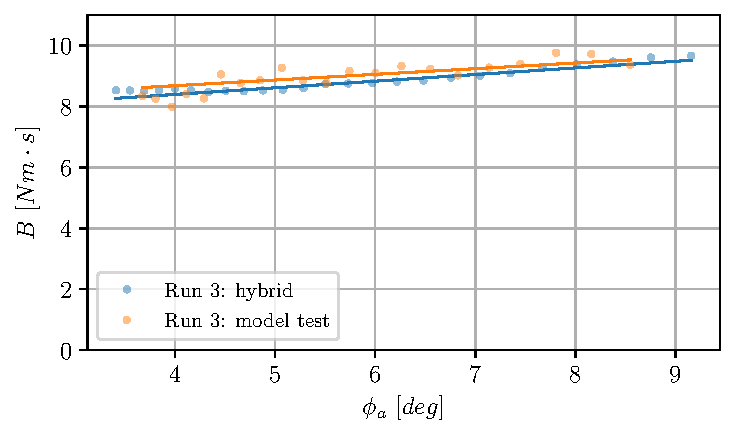
\includegraphics[width = 0.4\textwidth]{figures/hybrid_speed_amplitudes.pdf}\end{center}
        \vspace{-1cm}
        \caption{Total damping from Hybrid method (15.5 kn)}
        \label{fig:hybrid_speed_amplitudes}
    \end{figure}
    
The results using the Hybrid method for Run 3 at speed gives very
similar results to the corresponding model tests.

    \begin{figure}[H]
        \begin{center}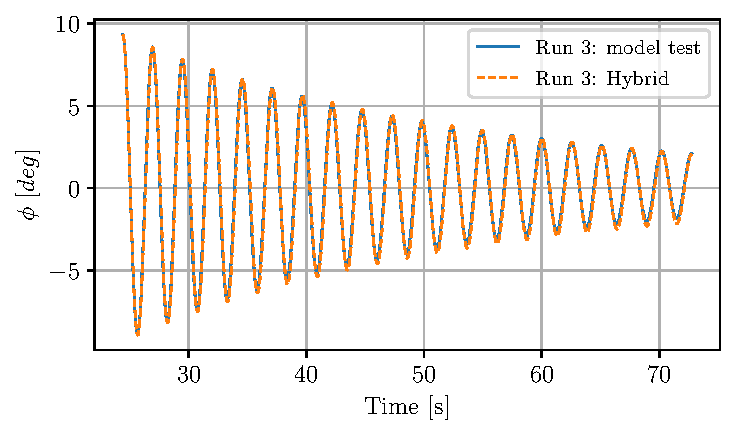
\includegraphics[width = 0.4\textwidth]{figures/hybrid_speed_time.pdf}\end{center}
        \vspace{-1cm}
        \caption{Roll decay with Hybrid method (15.5 kn)}
        \label{fig:hybrid_speed_time}
    \end{figure}
    
The coefficients obtained from model tests, FNPF and Hybrid method are summarized in model scale units in the table below:
 
            
\begin{table}[H]
\small
\center
\caption{Results}
\label{tab:results}
\begin{tabular}{lllllll}
\toprule\addlinespacerun & method & $F_n$ & $\omega_0$ & $B_1$ & $B_2$ & $B_3$\\ 
\midrule1 & model test & 0.0 & 2.4614 & 2.9604 & -6.5205 & 43.7754\\ 
2 & model test & 0.0 & 2.4611 & 2.8797 & -5.8742 & 41.5037\\ 
2 & FNPF & 0.0 & 2.4695 & 0.1425 & 2.9442 & 0.0\\ 
3 & model test & 0.1423 & 2.4675 & 7.5233 & 7.0281 & 0.3898\\ 
3 & FNPF & 0.1423 & 2.4418 & 7.5216 & 6.0148 & 0.0\\ 
\bottomrule
\end{tabular}
\end{table}
